\documentclass[11pt,a4paper]{article}
\usepackage{tikz}
\usepackage[legalpaper,margin=1in]{geometry}
\usetikzlibrary{positioning}
%include polycode.fmt
\begin{document}

\title {Marlowe: financial contracts on Cardano Computation Layer}
\author{Alexander Nemish}

\maketitle

\section{Introduction}

Here we present a reference implementation of Marlowe, domain-specific language targeted at
the execution of financial contracts in the style of Peyton Jones \emph{et al}
on Cardano Computation Layer.

The implementation is based on semantics described in paper
\emph{Marlowe: financial contracts on blockchain} by Simon Thompson and Pablo Lamela Seijas

We use PlutuxTx compiler, that compiles Haskell code into serialized \emph{Plutus Core} code,
to create a Cardano \emph{Validator Script} that secures value.

This \emph{Marlowe Validator Script} implements Marlowe interpreter, described in the paper.

\section{Extended UTXO model}
The \emph{extended UTxO model} brings a significant portion of the expressiveness of
Ethereum’s account-based scripting model to the UTxO-based Cardano blockchain.
The extension has two components: (1) an extension to the data carried by UTxO outputs
and processed by associated validator scripts together with
(2) an extension to the wallet backend to facilitate off-chain code
that coordinates the execution of on-chain computations.

\subsection{Extension to transaction outputs}
In the classic UTxO model (Cardano SL in Byron and Shelley),
a transaction output locked by a script carries two pieces of information:

\begin{itemize}
\item it’s value and
\item (the hash of) a validator script.
\end{itemize}

We extend this to include a second script, which we call the \emph{Data Script}.
This second script is a \emph{Plutus Core} expression, just like the \emph{Validator Script}.
However, the requirements on its type are different.
The type of the data script can be any monomorphic type.

\subsection{Extension to validator scripts}

An extended validator script expects four arguments:

\begin{itemize}
\item the redeemer expression,
\item the data script (from above),
\item the output’s value, and
\item parts of the validated transaction and related blockchain state. (More detail is in the next section.)
\end{itemize}

\begin{figure}[!h]
\centering
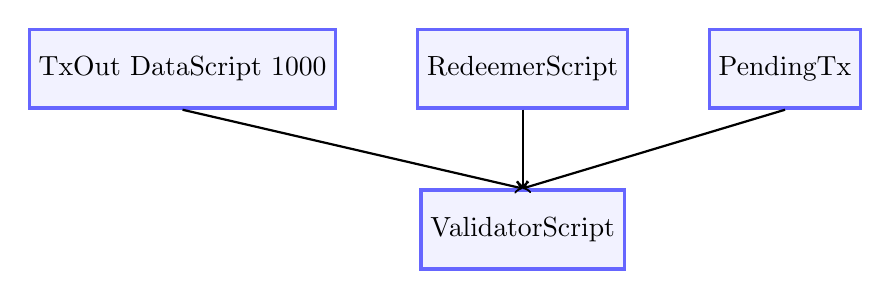
\begin{tikzpicture}[
squarednode/.style={rectangle, draw=blue!60, fill=blue!5, very thick, minimum size=10mm},
]
%Nodes
\node[squarednode] (txout) {TxOut DataScript 1000};
\node[squarednode] (txin) [right=of txout] {RedeemerScript};
\node[squarednode] (pedningTx) [right=of txin] {PendingTx};
\node[squarednode,align=center] (script)       [below=of txin] {ValidatorScript};

%Lines
\draw[->,thick] (txout.south) -- (script.north);
\draw[->,thick] (txin.south) -- (script.north);
\draw[->,thick] (pedningTx.south) -- (script.north);
\end{tikzpicture}
\end{figure}

We consider a validator script to have executed successful
if it does not terminate in the \emph{Plutus Core} \emph{error} state.

\subsection{Blockchain state available to validator scripts}

Validator scripts receive, at a minimum, the following information from the validated transaction
and the rest of the blockchain:

\begin{itemize}
\item the current block height (not including the currently validated transaction),
\item the hash of the currently validated transaction,
\item for every input of the validated transaction, its value and the hashes of its validator, data, and redeemer scripts,
\item for every output of the validated transaction, its value and the hash of its validator and data script, and
\item the sum of the values of all unspent outputs (of the current blockchain without the currently validated transaction) locked by the currently executed validator script.
\end{itemize}




\section{Assumptions}

\begin{itemize}
\item Fees are payed by transaction issues. For simplicity, assume zero fees.
\item Every contract is created by contract owner by issuing a transaction with the contract in TxOut
\end{itemize}



\section{Semantics}

Marlowe Contract execution is a chain of transactions,
where remaining contract and its state is passed through \emph{Data Script},
and actions/inputs (i.e. \emph{Choices} and \emph{Oracle Values}) are passed as
\emph{Redeemer Script}

\emph{Validation Script} is always the same Marlowe interpreter implementation, available below.

Both \emph{Redeemer Script} and \emph{Data Script} have the same structure:
\begin{spec} (Input, MarloweData) \end{spec}

where
\begin{itemize}
\item \emph{Input} contains contract actions (i.e. \emph{Pay}, \emph{Redeem}), \emph{Choices} and \emph{Oracle Values},
\item \emph{MarloweData} contains remaining \emph{Contract} and its \emph{State}
\item \emph{State} is a set of \emph{Commits} plus set of made \emph{Choices}
\end{itemize}

To spend TxOut secured by Marlowe Validator Script, a user must provide \emph{Redeemer Script}
that is a tuple of an \emph{Input} and expected output of Marlowe Contract interpretation for
the given \emph{Input}, i.e. \emph{Contract} and \emph{State}.

To ensure that user provides valid remainig \emph{Contract} and \emph{State}
\emph{Marlowe Validator Script} compares evaluated contract and state with provided by user,
and rejects a transaction if those don't match.

To ensure that remaining contract's \emph{Data Script} has the same \emph{Contract} and \emph{State}
as was passed with \emph{Redeemer Script}, we check that \emph{Data Script} hash is
the same as \emph{Redeemer Script}.
That's why those are of the same structure \begin{spec} (Input, MarloweData) \end{spec}.

\begin{figure}[!h]
\centering
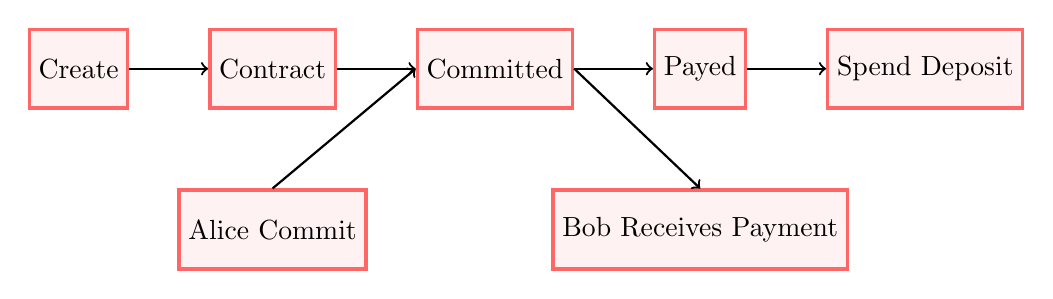
\begin{tikzpicture}[
squarednode/.style={rectangle, draw=red!60, fill=red!5, very thick, minimum size=10mm},
]
%Nodes
\node[squarednode,align=center] (deposit) {Create};
\node[squarednode,align=center] (c1) [right=of deposit] {Contract};
\node[squarednode,align=center] (c2) [right=of c1] {Committed};
\node[squarednode,align=center] (c3) [right=of c2] {Payed};
\node[squarednode,align=center] (c4) [right=of c3] {Spend Deposit};
\node[squarednode] (commit) [below=of c1] {Alice Commit};
\node[squarednode] (pay) [below=of c3] {Bob Receives Payment};

%Lines
\draw[->,thick] (deposit.east) -- (c1.west);
\draw[->,thick] (c1.east) -- (c2.west);
\draw[->,thick] (c2.east) -- (c3.west);
\draw[->,thick] (c3.east) -- (c4.west);
\draw[->,thick] (commit.north) -- (c2.west);
\draw[->,thick] (c2.east) -- (pay.north);
\end{tikzpicture}
\end{figure}


\subsection{Commit}

Alice has 1000 Ada.

\begin{figure}[!h]
\centering
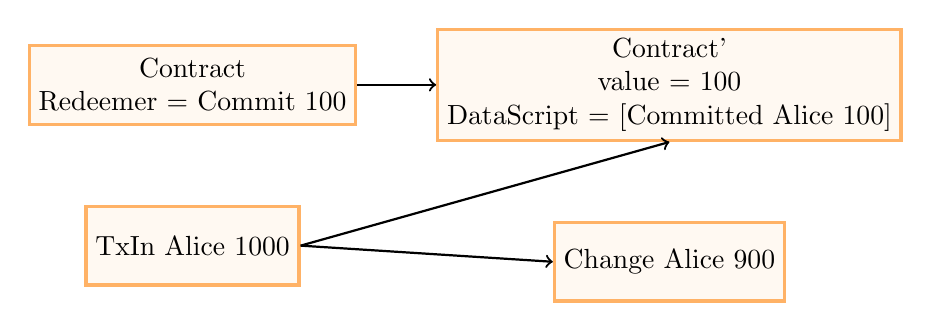
\begin{tikzpicture}[
squarednode/.style={rectangle, draw=orange!60, fill=orange!5, very thick, minimum size=10mm},
]
%Nodes
\node[squarednode,align=center] (contract) {Contract\\Redeemer = Commit 100};
\node[squarednode] (commitcash)  [below=of contract]
    {TxIn Alice 1000};
\node[squarednode,align=center] (txOut1)       [right=of contract]
    {Contract'\\value = 100\\DataScript = [Committed Alice 100]};
\node[squarednode] (txOut2)       [below=of txOut1]
    {Change Alice 900};

%Lines
\draw[->,thick] (contract.east) -- (txOut1.west);
\draw[->,thick] (commitcash.east) -- (txOut1.south);
\draw[->,thick] (commitcash.east) -- (txOut2.west);
\end{tikzpicture}
\end{figure}

\subsection{Redeem}

Redeem a previously make CommitCash if valid.
Alice committed 100 Ada with CC 1, timeout 256.

\begin{figure}[!h]
\centering
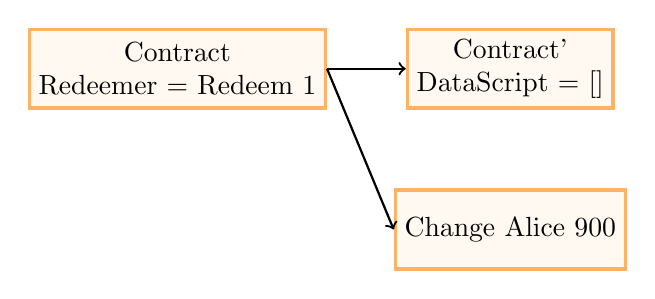
\begin{tikzpicture}[
squarednode/.style={rectangle, draw=orange!60, fill=orange!5, very thick, minimum size=10mm},
]
%Nodes
\node[squarednode,align=center] (contract) {Contract\\Redeemer = Redeem 1};
\node[squarednode,align=center] (txOut1)       [right=of contract]
    {Contract'\\DataScript = []};
\node[squarednode] (txOut2)       [below=of txOut1]
    {Change Alice 900};

%Lines
\draw[->,thick] (contract.east) -- (txOut1.west);
\draw[->,thick] (contract.east) -- (txOut2.west);
\end{tikzpicture}
\end{figure}

\subsection{Pay}

Alice pays 100 Ada to Bob.

\begin{figure}[!h]
\centering
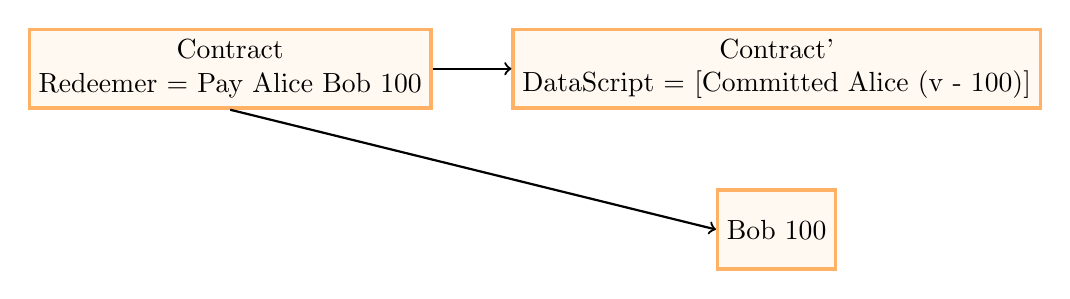
\begin{tikzpicture}[
squarednode/.style={rectangle, draw=orange!60, fill=orange!5, very thick, minimum size=10mm},
]
%Nodes
\node[squarednode,align=center] (contract) {Contract\\Redeemer = Pay Alice Bob 100};
\node[squarednode,align=center] (txOut1)       [right=of contract]
    {Contract'\\DataScript = [Committed Alice (v - 100)]};
\node[squarednode] (txOut2)       [below=of txOut1] {Bob 100};

%Lines
\draw[->,thick] (contract.east) -- (txOut1.west);
\draw[->,thick] (contract.south) -- (txOut2.west);
\end{tikzpicture}
\end{figure}


\subsection{SpendDeposit}

See \ref{ContractInit}

\section{Contract Initialization} \label{ContractInit}

This can be done in 2 ways.


\subsection{Initialization by depositing Ada to a new contract}

Just pay 1 Ada to a contract so that it becomes a part of \emph{eUTXO}.

\begin{figure}[!h]
\centering
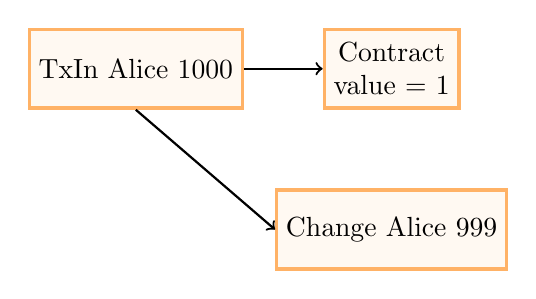
\begin{tikzpicture}[
squarednode/.style={rectangle, draw=orange!60, fill=orange!5, very thick, minimum size=10mm},
]
%Nodes
\node[squarednode] (commitcash) {TxIn Alice 1000};
\node[squarednode,align=center] (txOut1)       [right=of commitcash]
    {Contract\\value = 1};
\node[squarednode] (txOut2)       [below=of txOut1]
    {Change Alice 999};

%Lines
\draw[->,thick] (commitcash.east) -- (txOut1.west);
\draw[->,thick] (commitcash.south) -- (txOut2.west);
\end{tikzpicture}
\end{figure}


\par{Considerations}
Someone need to spend this 1 Ada, otherwise all Marlowe contracts will be in UTXO.
Current implementation allows anyone to spend this value.


\subsection{Initialization by CommitCash}

Any contract that starts with \emph{CommitCash} can be initialized with actuall \emph{CommitCash}

\begin{figure}[!h]
\centering
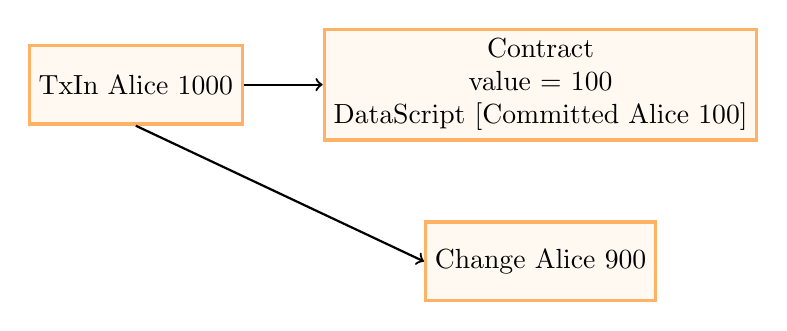
\begin{tikzpicture}[
squarednode/.style={rectangle, draw=orange!60, fill=orange!5, very thick, minimum size=10mm},
]
%Nodes
\node[squarednode] (commitcash) {TxIn Alice 1000};
\node[squarednode,align=center] (txOut1)       [right=of commitcash]
    {Contract\\value = 100\\DataScript [Committed Alice 100]};
\node[squarednode] (txOut2)       [below=of txOut1]
    {Change Alice 900};

%Lines
\draw[->,thick] (commitcash.east) -- (txOut1.west);
\draw[->,thick] (commitcash.south) -- (txOut2.west);
\end{tikzpicture}
\end{figure}
